\section{Duality}

\subsection{Lagrange dual function}

The Lagrangian dual function is always concave:
\begin{equation}
\begin{aligned}
g(\lambda,\mu) &= \underset{x \in D}{\text{inf}} L(x,\mu,\lambda)\\
&=\underset{x \in D}{\text{inf}}\Big(f_0(x) + \sum_i^m \lambda_i f_i(x) \sum_i^p\mu_i h_i(x)\Big)
\end{aligned}
\end{equation}
because this is the infimum over a set of affine functions. g is affine respect to x.
Now we get a \textbf{lower bound} if $\lambda \leq 0$ for our real function. 
$$f_0(\tilde{x} \geq L(\tilde{x}, \lambda, \mu) \geq inf(L) = g(\lambda,\mu) $$

basically if $\tilde{x}$ is feasible then $f_i$ is negative so the sum of non-negative numbers is negative. The product $h_i\mu$ is always 0 if x is feasible. Then we end up with a function that is always greater or equal than our original function, included the minimum of $f_0(x^*)$:
$$f_0(x^*)\geq g(\lambda,\mu)$$
\textbf{Very interesting, we got a lower bound. If we maximize g, which btw is concave.. then we get the best possible lower bound for our minimum of $f_0$}

Least-norm solution of linear set of equations. 
\minim{x^Tx}{Ax=b}
is basically constructing the dual Lagrangian function. Then minimize L. and g will give you a lower bound for the chosen $\lambda$.

So imagine the two way partitioning.
\minim{x^TWx}{x_i^2=1 \quad i = 1,2,..n}
Basically with the constraint you are enforcing the variables to be either 1 or -1 ( two classes) then with the cost function you are enforcing to put together the $x_ix_j$ that hate them the less $w_{ij}$. Or inversely, you put with different signs(class) the ones hate hate them the most. Ideally an even number of -1 and +1 is the best option. Every one -1 or +1 will add up in the cost function.. maximizing it the most. The more split the x vector the less cost function. The mos tseparated the ones that hate each other.. the less cost function. The only issue with this problem is that is non convex. An alternative would be:
\minim{x^TWx}{x_i^2\leq1}
where W is enforced to be positive defined
\subsubsection{Convex conjugate functions}
\url{https://www.slideshare.net/ryotat/convex-optimization-old-tricks-for-new-problems}
The convex conjugate function of a set is
$$f^*(y) = \underset{x \in dom(f)}{sup}(y^Tx -f(x))$$
Conjugate functions are a way to create a convex hull of the epigraph of our cost function, $f_0$. Conjugate functions are convex even when the cost function is not. 

\begin{figure}
\centering
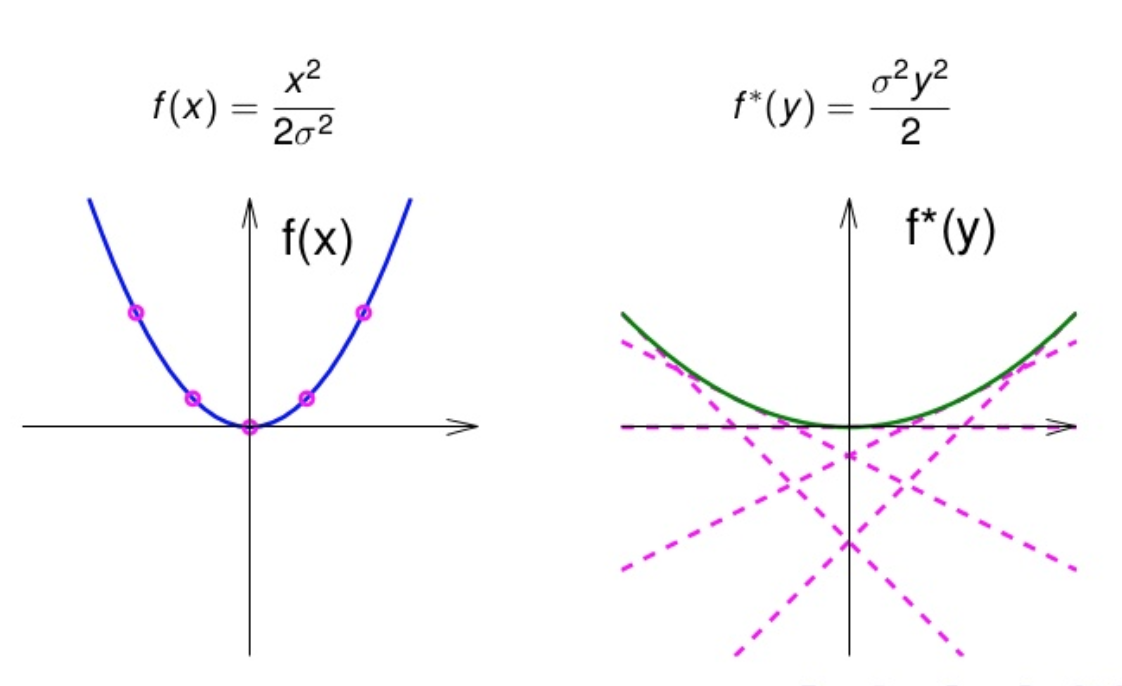
\includegraphics[width=0.6\textwidth]{images/conjugate.png}
\caption{\label{fig:frog}conjugate of parabola}
\end{figure}

\subsection{The Lagrange dual problem}
The dual function,$g(\lambda,\nu)$, of our original cost function, $f_0$, gives us a parametrize lower bound of the optimal point $p*$. 
Which one is the best lower bound? The following problem leads to the solution.
\maxim{g(\lambda,\nu)}{\lambda \geq 0}
This problem is called \textit{the Lagrange dual problem}. Remember that $\lambda$ should be negative since the constraint $f_i$ is always negative if the points are feasible, while the sign of $\nu$ does not matter since $h_i$ is 0 when feasible. In order to be feasible, the dual problem, must have $g(\lambda,\nu)>-\infty$ and $\lambda>0$. 
\textbf{The dual problem is always a convex problem}, so lower bounds for $p*$ can be calculated even for non-convex problems. The objective is concave while the inequality constraint is convex.

\subsection{Making dual implicit constraints explicit}
Imagine the following problem,
\minimall{c^Tx}{Ax=b}{x\succeq 0}
the dual function hence looks like
\begin{equation}
\begin{aligned}
\text{inf} \quad L(x,\lambda,\nu)&=\text{inf} \quad (c+A^T\nu-\lambda)x - b^T\nu \\
& g(\lambda,\nu) = -b^T \nu \quad \text{if} \quad c+A^T\nu-\lambda = 0 \quad -\infty \quad \text{otherwise}
\end{aligned}
\end{equation}
The dual problem then would be
\maxim{g(\lambda,\nu)}{\lambda \succeq 0}
but if we take in account the constraints in the domain in order to have a feasible dual problem, we should incorporate the implicit constraints
\maximall{-b^T\nu}{c+A^T\nu-\lambda=0}{\lambda \succeq 0}
which can be simplify as 
\maxim{-b^T}{c+A^T\nu \succeq 0}
\subsubsection{Strong and Weak duality: Slaters Qualifications}
When $d*<p*$ then weak duality holds. We define the duality gap as $p*-d*$. In case that $p*=-\infty$ then $d*=-\infty$ which means that the dual problem is unfeasible. Conversely, if $d*=\infty$ then $p*=\infty$ which means that the \textit{primal problem} is unfeasible.\\
When $p*=d*$ \textit{strong duality holds} and this holds generally when the problem is convex, but not always. Further conditions must be satisfy, the \textit{Slaters qualifications}: there must be some x  feasible
\begin{equation}
f_i(x) < 0 \qquad i = 1,2,...,m, \qquad Ax = b
\end{equation}
which can be relaxed when the inequalities are affine to
\begin{equation}
f_i(x) < 0 \qquad i = 1,2,...,m, \qquad Ax = b
\end{equation}
which is the same than saying that \textbf{the problem is feasible}. Awesome! proof will be given later. Let's see an example:
\minim{x^Tx}{Ax=b}
then the Lagrange function 
\begin{equation*}\begin{aligned}
L(x,\nu)&=x^Tx +(Ax-b)^T\nu\\
\end{aligned}\end{equation*}
\begin{equation*}\begin{aligned}
\frac{L(x,\nu)}{dx} &= 2x + A^T\nu = 0\\
x &= -A\nu/2
\end{aligned}\end{equation*}
hence the dual function
\begin{equation*}
\begin{aligned}
g(\nu) &= (-A^T\nu/2)^T(-A^T\nu/2) + (A(-A^T\nu/2) - b)^T\nu\\
&=(1/4)\nu^TAA^T\nu - (1/2)(A^T\nu)^TA^T\nu -b^T\nu \\
&=(1/4)\nu^TAA^T\nu - (1/2)\nu^TAA^T\nu -b^T\nu \\
&=-(1/4)\nu^TAA^T\nu -b^T\nu \\
\end{aligned}
\end{equation*}
here Slater qualifications are fulfill when the primal problem is feasible i.e. $b\in R(A)$ and $p*<\infty$. CHECKOUT IN CASE THAT $p*=\infty$
\textcolor{red}{check also the zero sum game case from 5.2.5}
\subsection{Geometric Interpretation}
Imagine all the possible values that the objective,$f_0(x)$, and the constraint functions,$f_m(x)$ and $h_p(x)$ can take. It can be expressed with the following set:
$$\mathbb{G} =\{(f_1(x)...f_m(x),h_1(x)...h_p(x),f_0)\in \mathbb(\mathbb{R}^m\times\mathbb{R}^p\times\mathbb{R} | x \in \mathbb{D}\}$$
then we denote the optimal value as
$$p* = \text{inf}\{t | (u,v,t) \in \mathbb{G},\quad u \succeq 0,\quad v=0\}$$
The Lagrange function can be expressed as 
$$L(x,\lambda,\nu) = (\lambda,\nu,1)^T(u,v,t) $$
and the dual function as
$$g(\lambda,\nu) = inf\{(\lambda,\nu,1)^T(u,v,t) \in \mathbb{G}\}$$
then the following inequality holds...
$$(\lambda,\nu,1)^T(u,v,t)\geq g(\lambda,\nu)$$
which basically means that there a supporting hyperplane to $\mathbb{G}$ in the point (u,v,t). My point of view: you calculate the minimum of the Lagrangian and this gives you a parametrize hyperplane $\lambda u + t = g(lambda)$. Then by choosing a slope $\lambda$ you push the hyperplane as close to the $\mathbb{G}$.. and that give you $g(\lambda)$ in the intersection with the axis. 

\begin{figure}
\centering
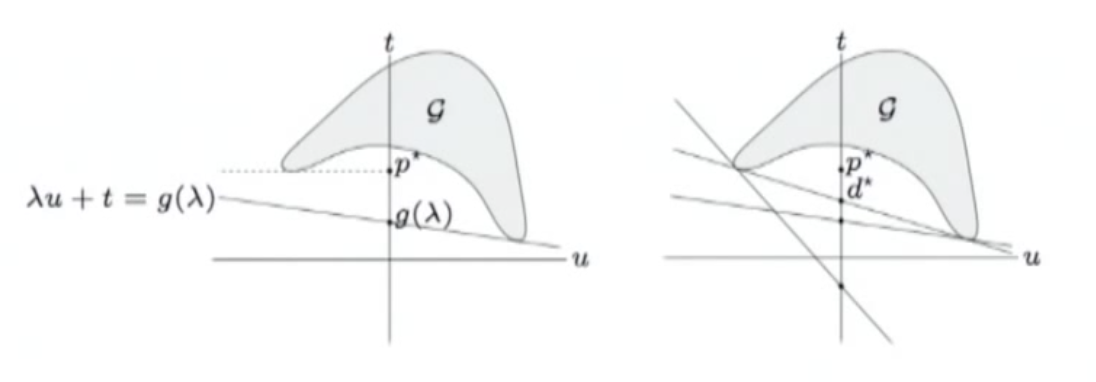
\includegraphics[width=1\textwidth]{images/supporthyperplanes.png}
\caption{Supporting hyperplanes}
\end{figure}
\subsubsection{Poof of strong duality}
\subsection{Optimality conditions}
\subsubsection{Complementary slackness}
Suppose that strong duality holds then x* is primal optimal and $(\lambda^*,\nu^*)$ are dual optimal
\begin{equation*}\begin{aligned}
f_0(x^*)=g(\lambda^*,\nu^*) &= \text{inf}\{ f_0(x) + \sum_{i=0}^N \lambda_i^*f_i(x) + \sum_{i=0}^p \nu_i^* h_i(x) \\
&\leq f_0(x^*) + \sum_{i=0}^N \lambda_i^*f_i(x^*) + \sum_{i=0}^p \nu_i^* h_i(x^*)\\
&\leq f_0(x^*)
\end{aligned}
\end{equation*}
Basically, the original function evaluated in the optimal point is equal to the dual evaluated in the dual optimal. The latter is equal to the infimum of the Lagrange function which less or equal than the Lagrangian which is less or equal than the original function. However, if we follow the chain, we can see that $$f_0(x^*)\leq f_0(x^*)$$ is only valid if they are actually equal. Ten all the inequalities actually are equalities. 
$$\leq f_0(x^*) + \sum_{i=0}^N \lambda_i^*f_i(x^*) + \sum_{i=0}^p \nu_i^* h_i(x^*) = \leq f_0(x^*)$$
We see that if x is feasible the $\nu*h_(x)$ is 0. However in order to satisfy the the equation also $f_i(x*)\lambda_i=0$ should be satisfied. This condition called \textbf{complementary slackness} 
\subsubsection{KKT conditions}
Now we are prepared to enumerate the KKT conditions for a convex problem where strong duality holds:
\begin{itemize}
\item Primal constraint: $f_i(x^*)\leq0$ and $h_i(x^*) = 0$
\item Dual constraint: $\lambda \succeq 0$
\item complementary slackness: $f_i(x^*)\lambda_i = 0$ for $i=1,\dots, m.$
\item gradient of Lagrangian should vanish: $\nabla f_0(x^*)+\sum^m\lambda_i\nabla f_i(x^*)+\sum^p\nu_i\nabla h_i(x^*) = 0$
\end{itemize}
The latter is true since the $x^*$ is the point that minimize the Lagrangian and gives us the dual function. Since the Lagrangian is a convex function, the gradient must be zero in the optimal point( you can not go further down or up)
\subsubsection{Mechanical interpretation of KKT conditions}
